\documentclass{article}
\usepackage[utf8]{inputenc}
\usepackage[T1]{fontenc}
\usepackage[ukrainian]{babel}
\usepackage[12pt]{extsizes}
\usepackage{graphicx}
\usepackage{amsmath}
\usepackage{amsfonts}
\usepackage{multicol}
\usepackage{cmap}
\usepackage{amsthm}
\graphicspath{{pictures/}}
\DeclareGraphicsExtensions{.pdf,.png,.jpg}

%ABC

\title{Теорвер}
\author{nikita.forduy }
\date{February 2020}

\usepackage{natbib}
\usepackage{graphicx}

\begin{document}
\pagestyle{empty}
\newtheorem{theorem}{Теорема}

\begin{titlepage}
    \thispagestyle{empty}
    \setlength{\parindent}{0ex} % set paragraph indenting to zero
    
    \begin{center}
      НАВЧАЛЬНО-НАУКОВИЙ КОМПЛЕКС \\
      "ІНСТИТУТ ПРИКЛАДНОГО СИСТЕМНОГО АНАЛІЗУ" \\
      НАЦІОНАЛЬНОГО ТЕХНІЧНОГО УНІВЕРСИТЕТУ УКРАЇНИ \\
      "КИЇВСЬКИЙ ПОЛІТЕХНІЧНИЙ ІНСТИТУТ ІМЕНІ ІГОРЯ СІКОРСЬКОГО" \\
      \smallskip
      КАФЕДРА МАТЕМАТИЧНИХ МЕТОДІВ СИСТЕМНОГО АНАЛІЗУ \\
    \end{center}
    \vspace{60mm}
    
    \begin{center}
      РОЗРАХУНКОВА РОБОТА \\
      з предмету "Математична статистика" \\
    \end{center}
    
    \vspace{30mm}
    

    \hfill
    \begin{minipage}{.4\linewidth}
      \begin{flushright}
        Виконав студент групи КА-81
        Фордуй Нікіта
        \smallskip
        Перевірила Каніовська І.Ю.
      \end{flushright}
    \end{minipage}
    
    \vspace{10mm}

    \vfill
    \begin{center}
      Київ 2020
    \end{center}
    
    \setlength{\parindent}{5ex} % reset paragraph indenting
\end{titlepage}

\pagestyle{plain}

\large
\section{Завдання}
Дана конкретна реалізація вибірки об’ємом n = 100:
\newline
\newline
\begin{tabular}{cccccccccccccccccccc}
  \ttfamily 2 & 0 & 8 & 0 & 15 & 1 & 1 & 1 & 7 & 1 & 0 & 0 & 
  3 & 1 & 1 & 1 & 0 & 0 & 3 & 1 \\
  \ttfamily 2 & 4 & 10 & 6 & 1 & 0 & 1 & 0 & 0 & 2 & 0 & 1 & 
  5 & 0 & 1 & 9 & 4 & 2 & 11 & 3\\
  \ttfamily 2 & 0 & 8 & 1 & 6 & 3 & 0 & 1 & 1 & 4 & 0 & 9 & 
  5 & 3 & 3 & 0 & 0 & 10 & 2 & 0\\
  \ttfamily 3 & 11 & 0 & 9 & 0 & 1 & 4 & 1 & 0 & 2 & 0 & 1 & 
  1 & 3 & 4 & 7 & 1 & 3 & 3 & 0 \\
  \ttfamily 4 & 7 & 6 & 0 & 3 & 0 & 1 & 15 & 11 & 1 & 2 & 4 & 
  0 & 2 & 0 & 0 & 0 & 26 & 4 & 0
\end{tabular}
\begin{enumerate}
  \item Побудувати варіаційний (дискретний або інтервальний) ряд наданої вибірки.
  \item Зробити графічне зображення вибірки.
  \item Побудувати емпіричну функцію розподілу.
  \item Обчислити значення вибіркової медіани, моди, асиметрії.
  \item Знайти незміщену оцінку математичного сподівання та дисперсії.
  \item Висунути гіпотезу про розподіл, за яким отримано вибірку.
  \item Знайти точкові оцінки параметрів гіпотетичного закону розподілу та перевірити їх властивості.
  \item Перевірити за допомогою критерію $\chi^2$ (Пірсона) гіпотезу про розподіл з рівнем значущості $\alpha$ = 0,05.
  \item Знайти довірчий інтервал для параметрів гіпотетичного закону розподілу, взяв рівень надійності $\gamma = 0.95$.
  \item Висновки.
\end{enumerate}
\section{Побудова варіаційного ряду вибірки }
Маємо невелику кількість різних значень - тому побудуємо 
дискретний варіаційний ряд.
Підрахувавши кількість варіант (14) та їх частоти і знаючи 
об’єм вибірки побудуємо 
дискретний варіаційний ряд :
\newline
\newline
\begin{tabular}{|p{44pt}|p{13pt}|p{13pt}|p{13pt}|p{13pt}
  |p{13pt}|p{13pt}|p{13pt}|p{13pt}|p{13pt}|p{13pt}|p{13pt}
  |p{13pt}|p{13pt}|p{13pt}|}
  \hline
  $x_i^*$& 0 & 1 & 2 & 3 & 4 & 5 & 6 & 7 & 8 & 9 & 10 & 11 & 15 & 26\\
  \hline
  $n_i$& 29 & 22 & 9 & 11 & 8 & 2 & 3 & 3 & 2 & 3 & 2 & 3 & 2 & 1\\
  \hline
  $\omega_i = \frac{n_i}{n}$ & $\frac{29}{100}$ & 
  $\frac{22}{100}$ & $\frac{9}{100}$ & $\frac{11}{100}$ & 
  $\frac{8}{100}$ & $\frac{2}{100}$ & $\frac{3}{100}$ 
  & $\frac{3}{100}$ & $\frac{2}{100}$ & $\frac{3}{100}$ & 
  $\frac{2}{100}$ & $\frac{3}{100}$ & $\frac{2}{100}$ & 
  $\frac{1}{100}$\\
  \hline
  $\omega_i^H$&$\frac{29}{100}$&$\frac{51}{100}$&$\frac{60}{100}$&
  $\frac{71}{100}$&$\frac{79}{100}$&$\frac{81}{100}$&$\frac{84}{100}$&
  $\frac{87}{100}$&$\frac{89}{100}$&$\frac{92}{100}$&$\frac{94}{100}$&
  $\frac{97}{100}$&$\frac{99}{100}$&1\\
  \hline
\end{tabular}
\newline
\newline
де $x_i^*$ - варіанти, $n_i$ - частота i-тої 
варіанти, $\omega_i = \frac{n_i}{n}$ - частість i-тої варіанти або 
відносна частота, $\omega_i^H$ - накопичена частість i-тої варіанти.
\newline
За дискретним варіаційним рядом побудуємо його геометричну 
інтерпретацію - полігон частостей:
\newline
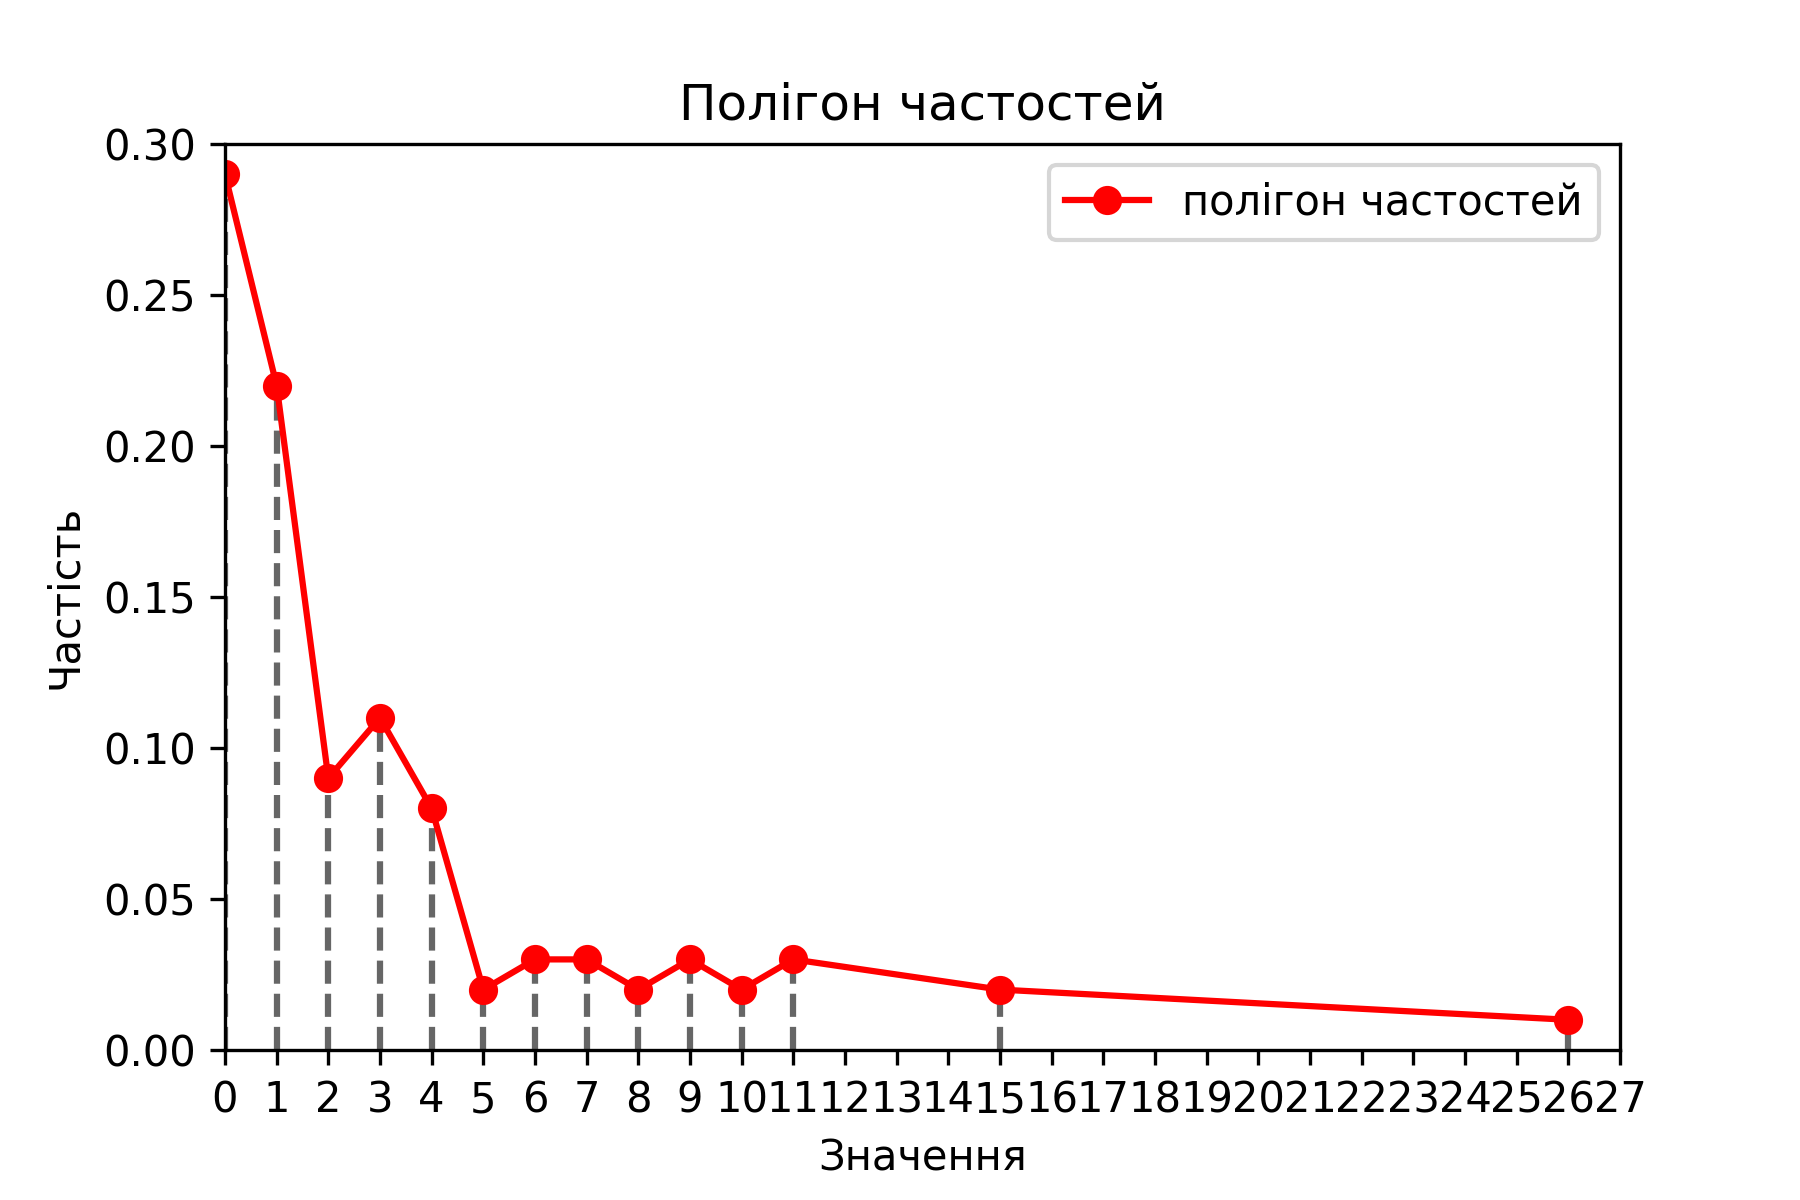
\includegraphics[scale = 0.9]{pol}
Порівняємо полігон частостей нашої реалізації 
вибірки із полігоном ймовірностей закону Паскаля при 
різних значеннях його параметра.
\newline
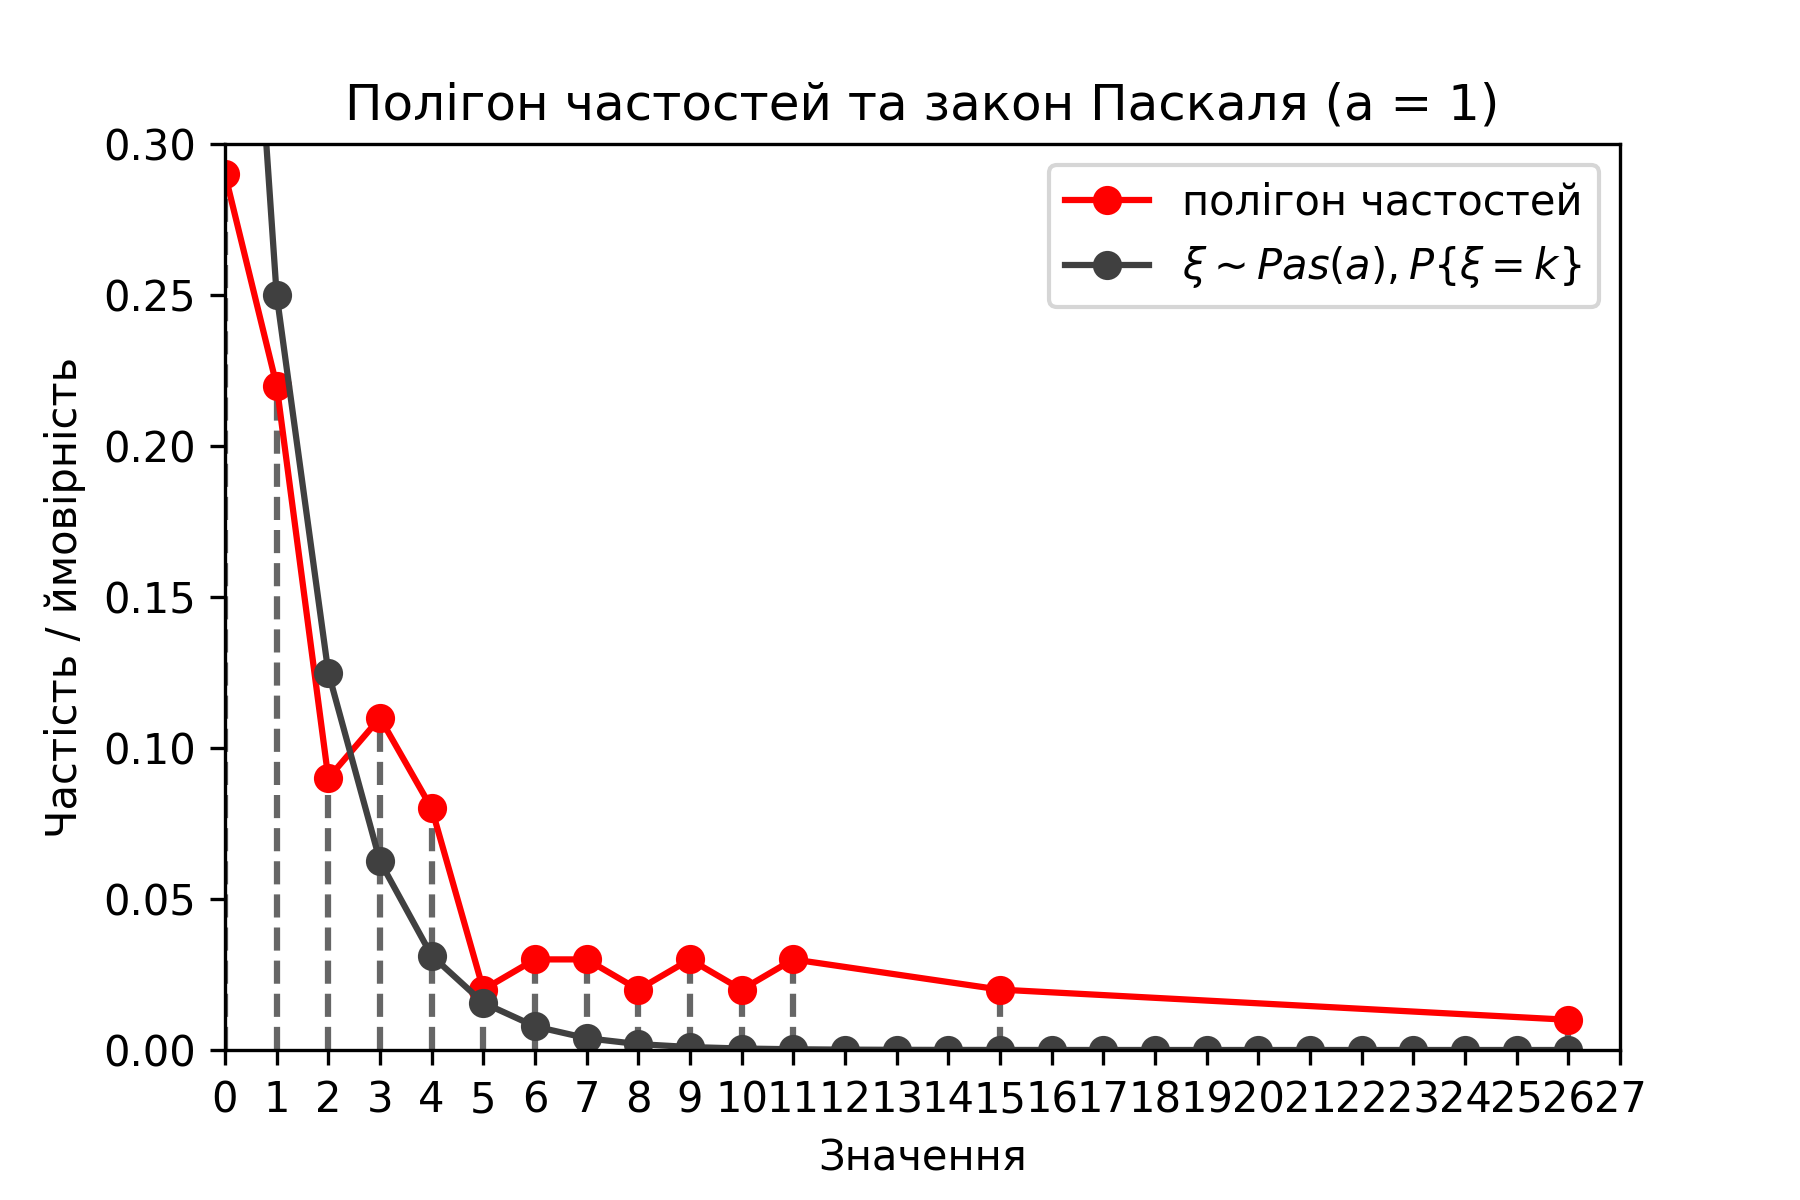
\includegraphics[scale = 0.8]{pol+pas1}
\newline
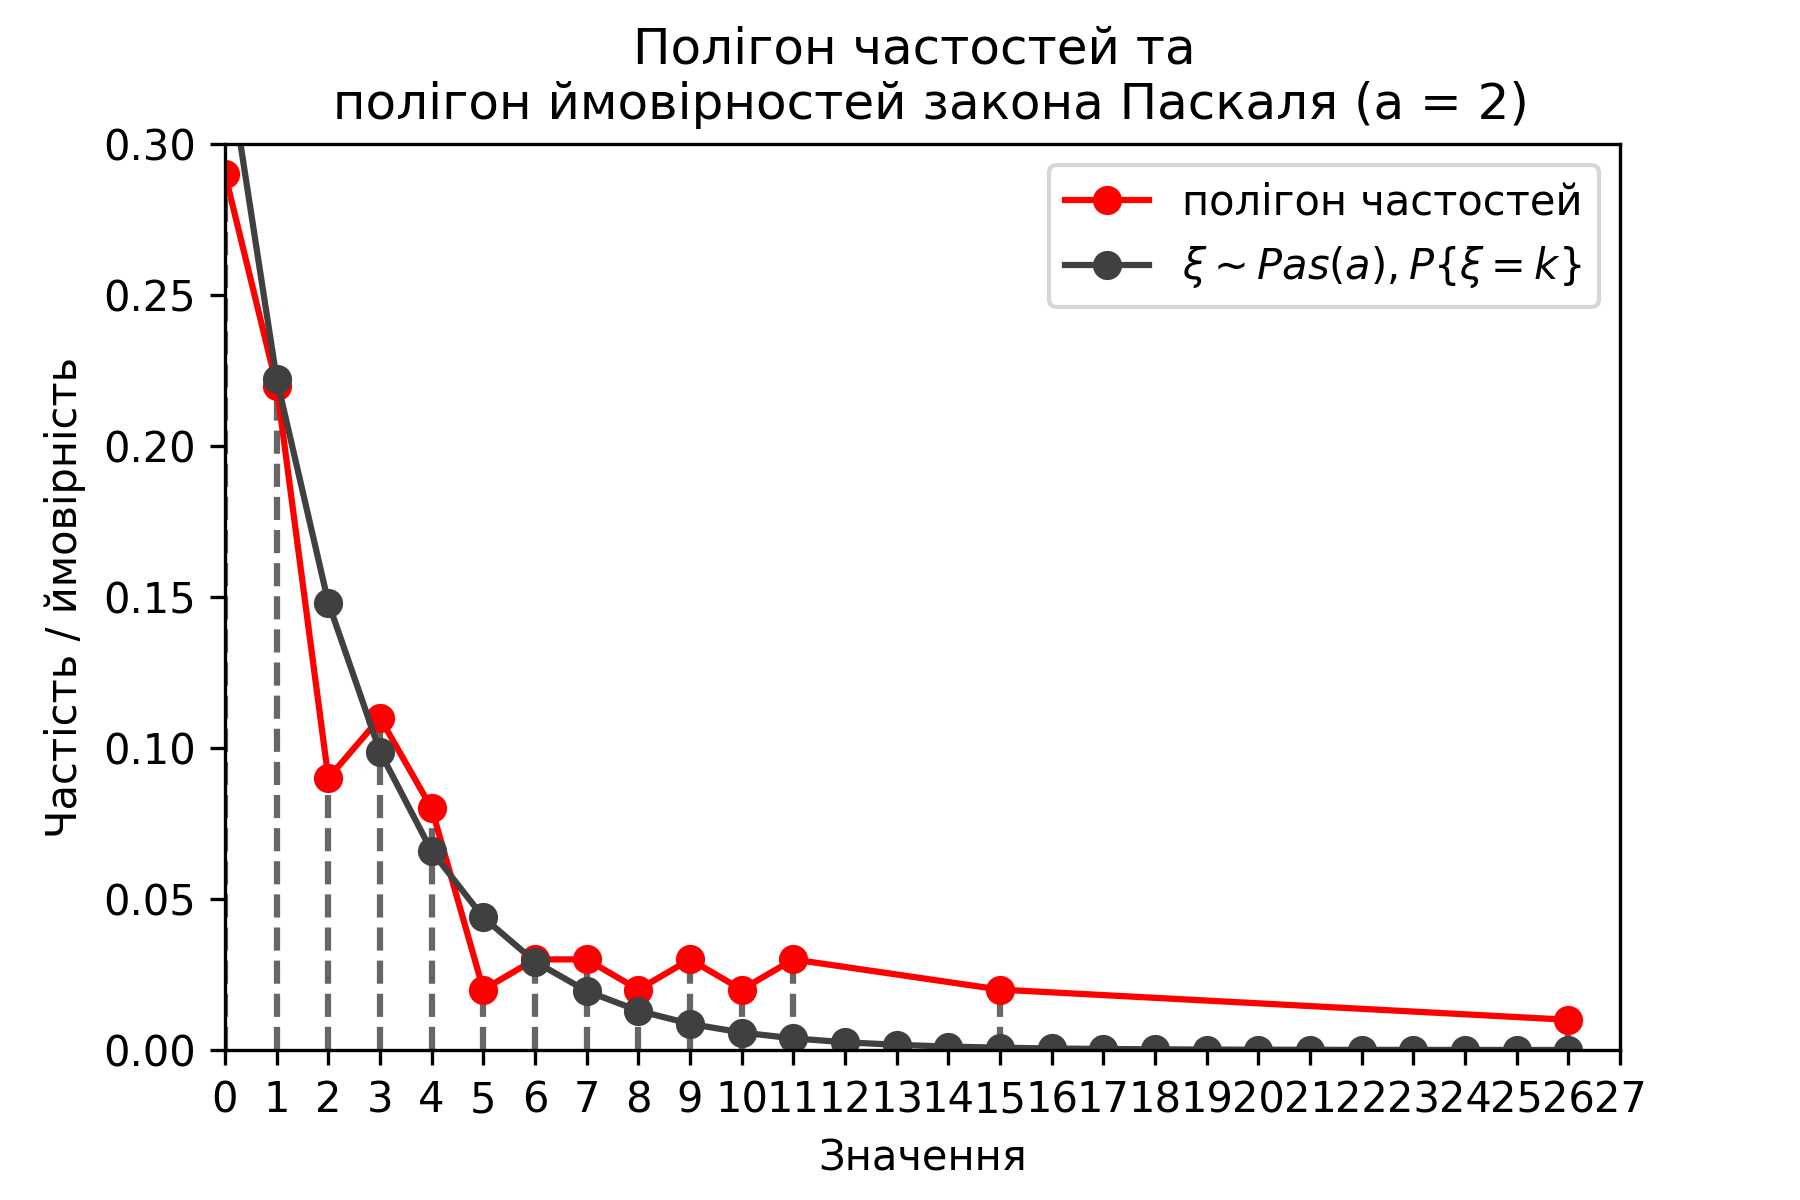
\includegraphics[scale = 0.8]{pol+pas2}
\newline
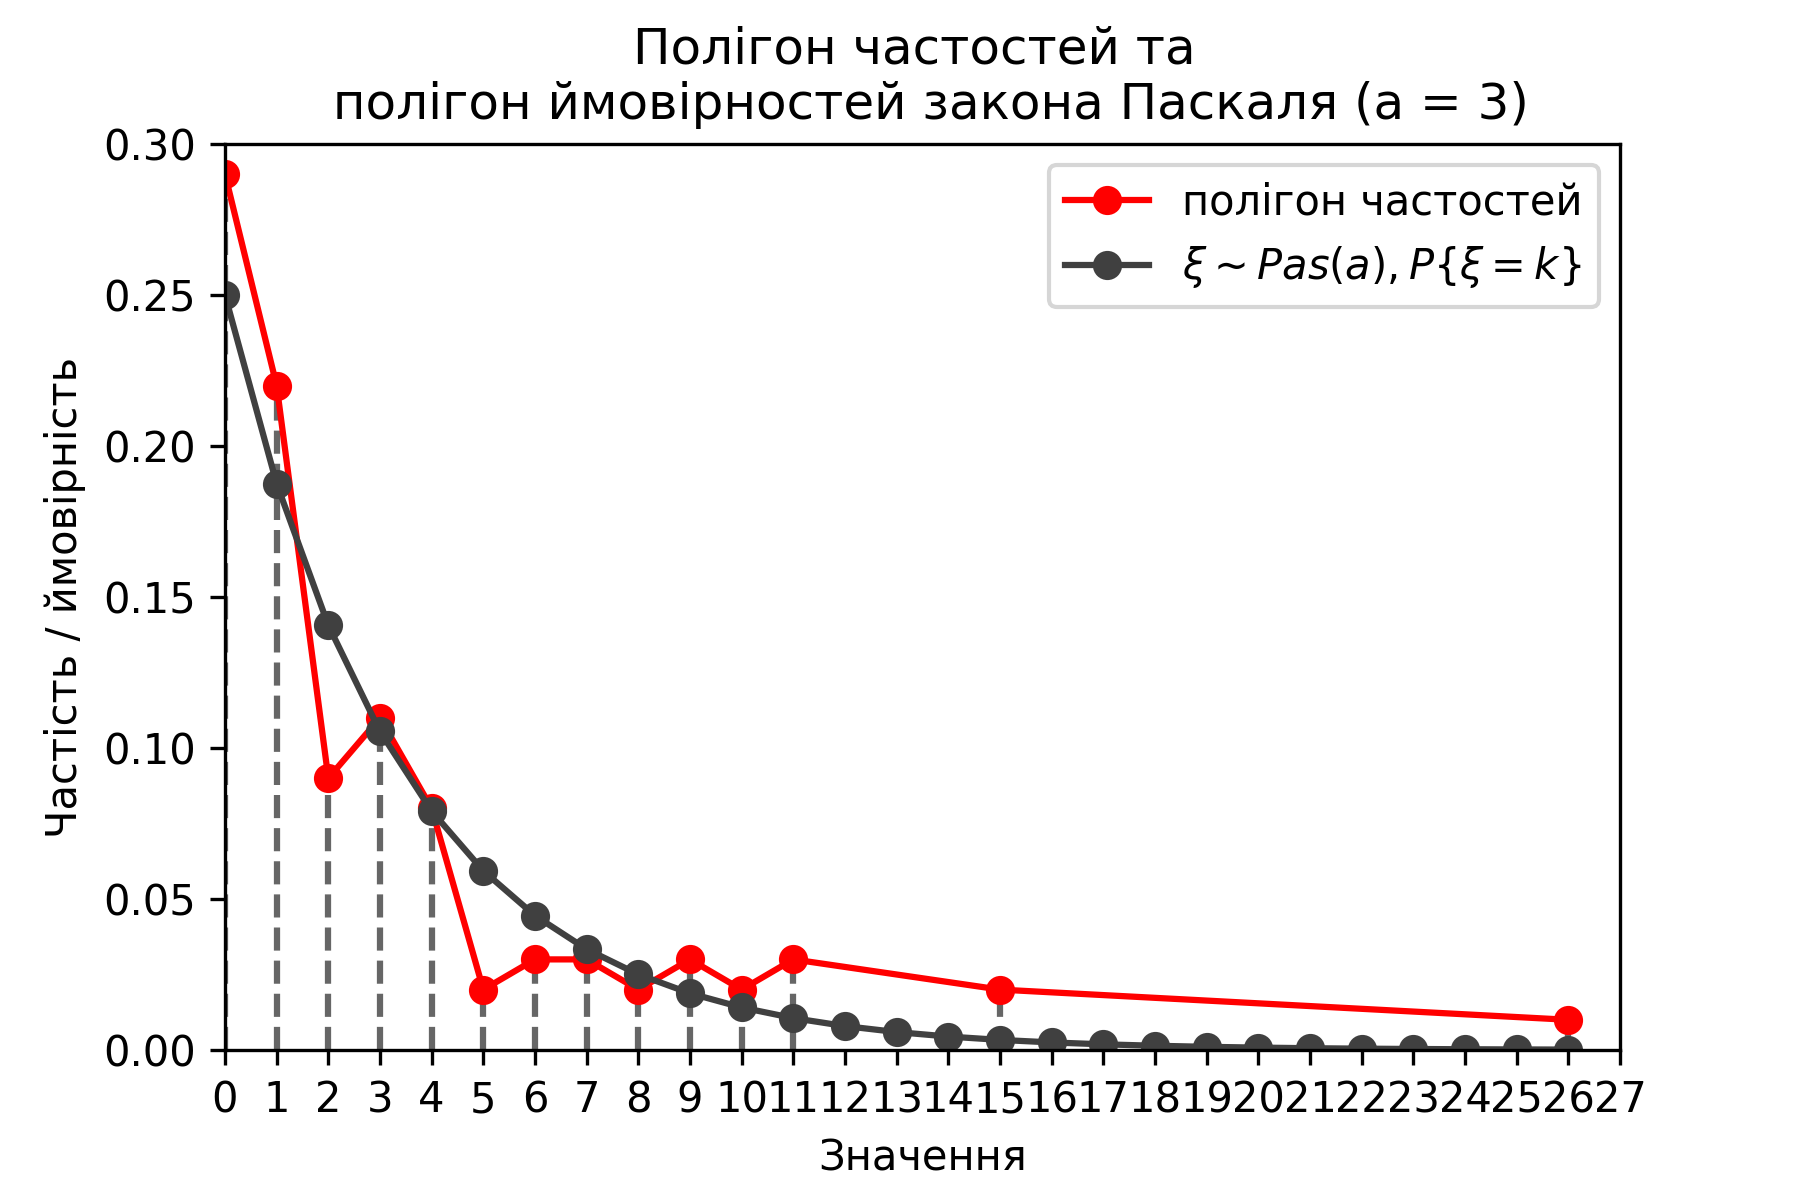
\includegraphics[scale = 0.8]{pol+pas3}
\newline
Можна зауважити, що полігон ймовірностей закону Паскаля
при певних значеннях його параметра (a = 1, 2, 3) 
достатньо схожий на полігон частостей нашої реалізації вибірки.
\newpage
\section{Емпірична функція розподілу}
Побудуємо емпіричну функцію розподілу за вже побудованим 
дискретним варіаційним рядом:
\newline
\begin{equation}
  F_n^*(x) = \begin{cases}
    0,  & x \leq 0 \\
    \frac{29}{100}, & 0 < x \leq 1 \\
    \frac{29 + 22}{100} = \frac{51}{100}, & 1 < x \leq 2 \\
    \frac{51}{100} + \frac{9}{100} = \frac{60}{100}, & 2 < x \leq 3 \\
    \frac{60}{100} + \frac{11}{100} = \frac{71}{100}, & 3 < x \leq 4 \\
    \frac{71}{100} + \frac{8}{100} = \frac{79}{100}, & 4 < x \leq 5 \\
    \frac{79}{100} + \frac{2}{100} = \frac{81}{100}, & 5 < x \leq 6 \\
    \frac{81}{100} + \frac{3}{100} = \frac{84}{100}, & 6 < x \leq 7 \\
    \frac{84}{100} + \frac{3}{100} = \frac{87}{100}, & 7 < x \leq 8 \\
    \frac{87}{100} + \frac{2}{100} = \frac{89}{100}, & 8 < x \leq 9 \\
    \frac{89}{100} + \frac{3}{100} = \frac{92}{100}, & 9 < x \leq 10 \\
    \frac{92}{100} + \frac{2}{100} = \frac{94}{100}, & 10 < x \leq 11 \\
    \frac{94}{100} + \frac{3}{100} = \frac{97}{100}, & 11 < x \leq 15 \\
    \frac{97}{100} + \frac{2}{100} = \frac{99}{100}, & 15 < x \leq 26 \\
    \frac{99}{100} + \frac{1}{100} = 1, & x > 26 \\
  \end{cases}
\end{equation}
\newpage
Зобразимо емпіричну функцію розподілу геометрично :
\newline
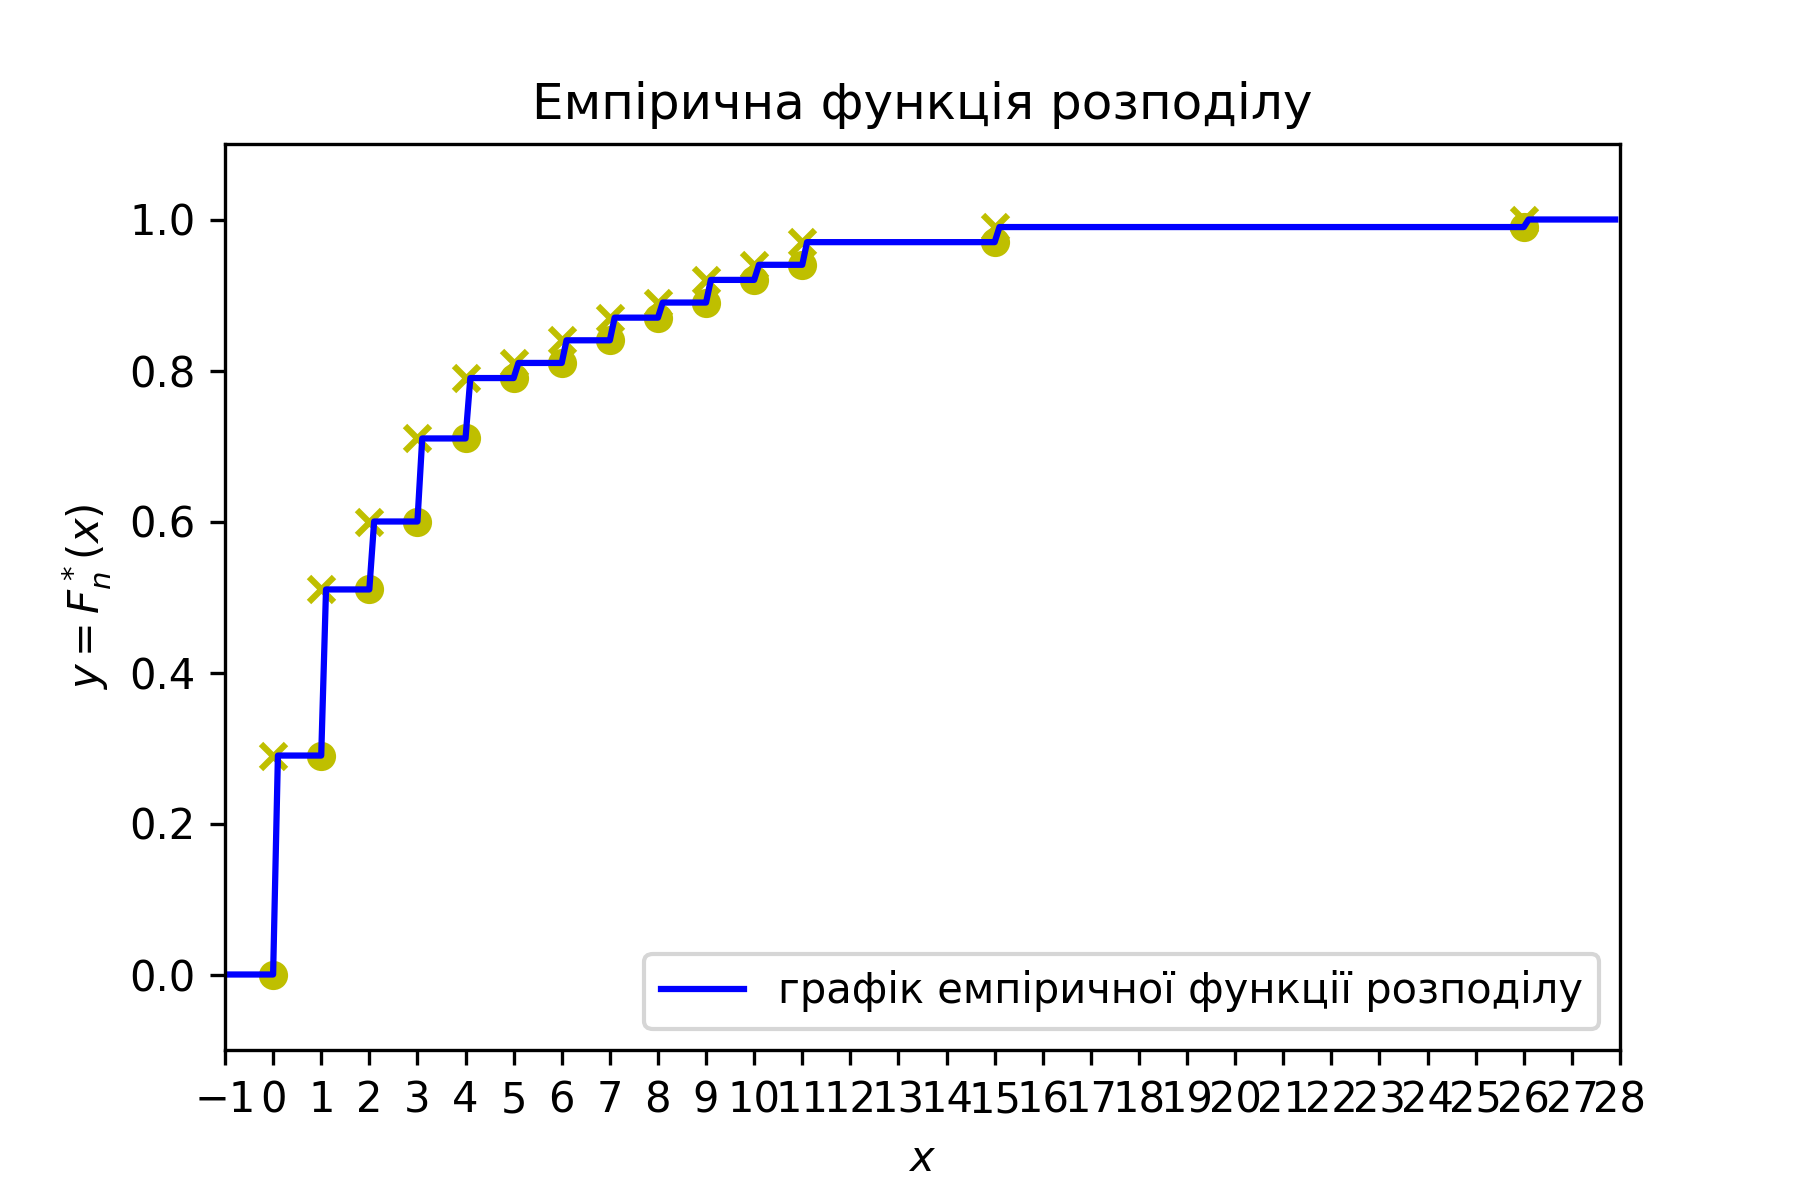
\includegraphics[scale = 0.8]{func}
\newline
Порівняємо графік емпіричної функції розподілу варіаційного ряду 
з графіком функції розподілу закону Паскаля при 
різних параметрах(a = 1, 2, 3):
\newline
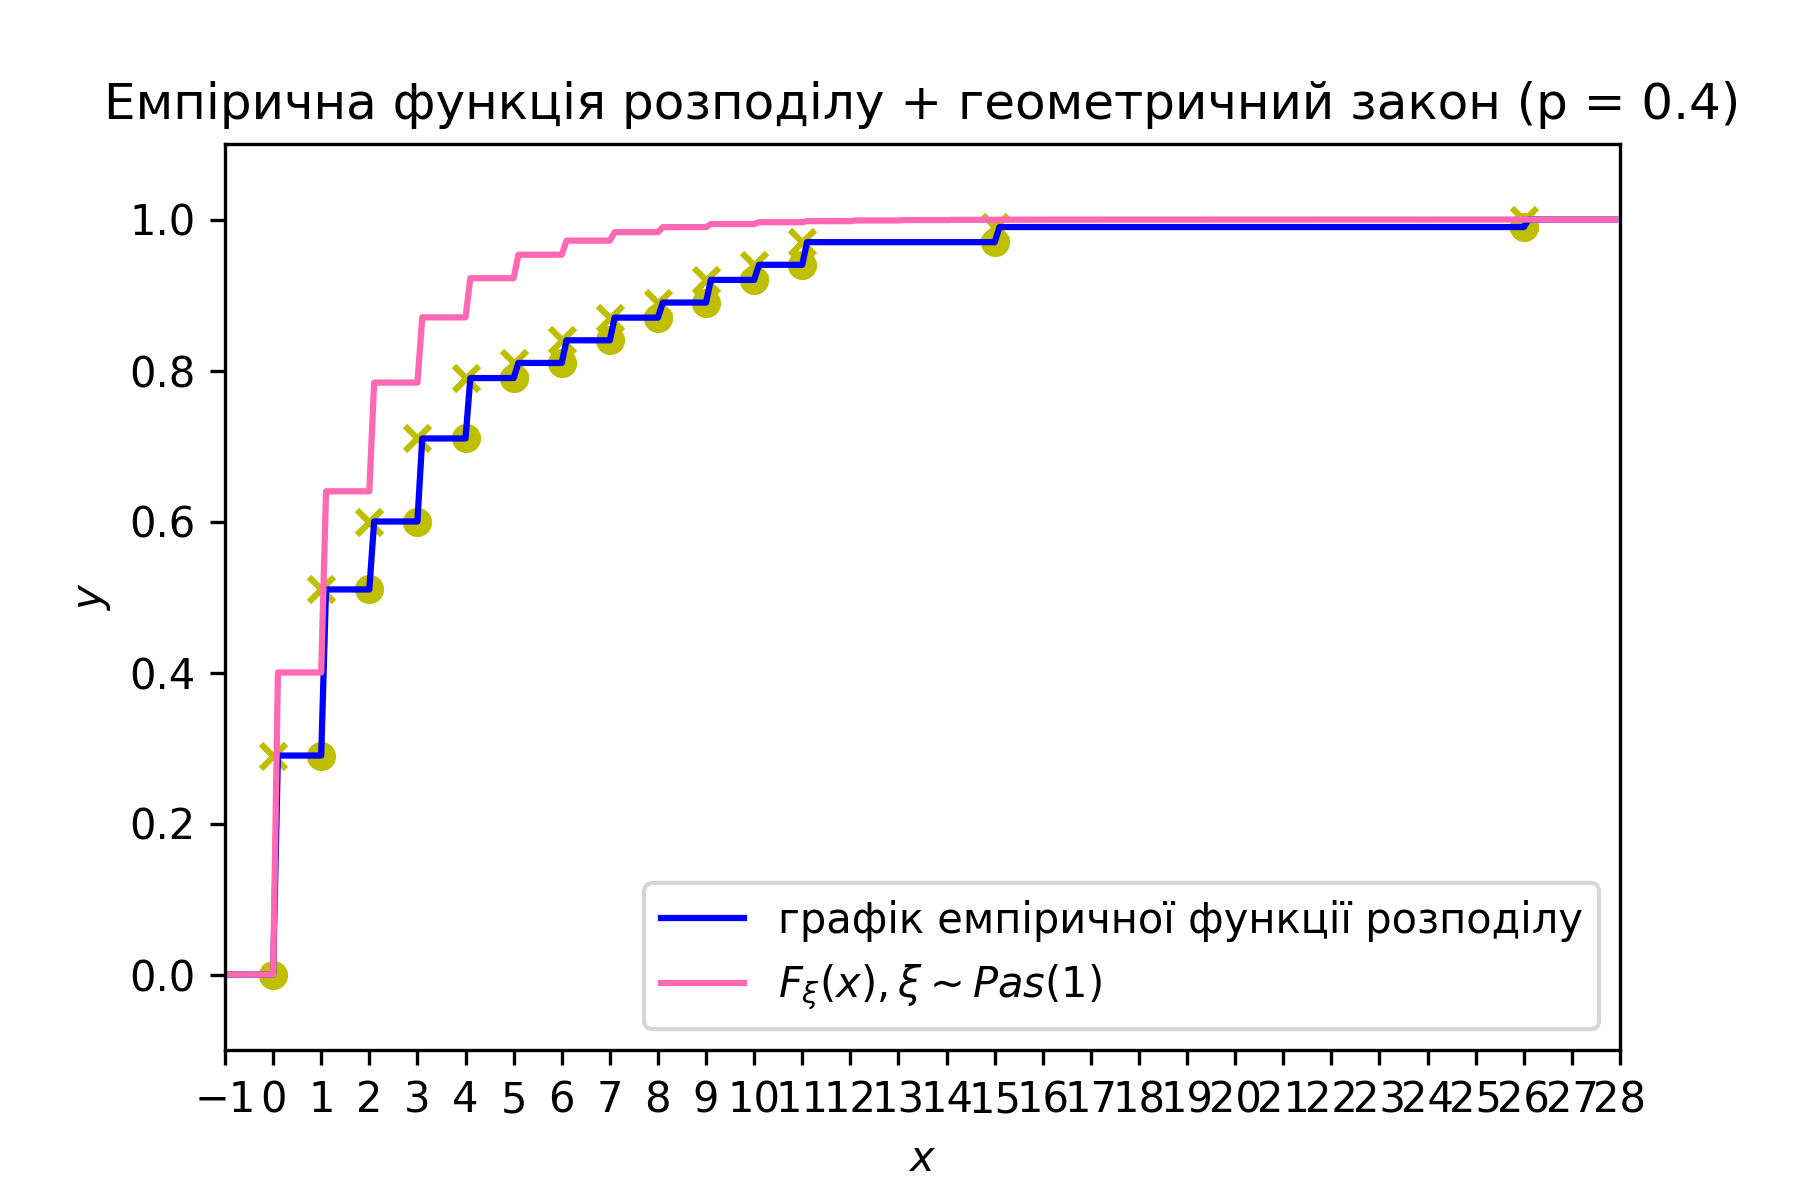
\includegraphics[scale = 0.8]{func+geom4}
\newline
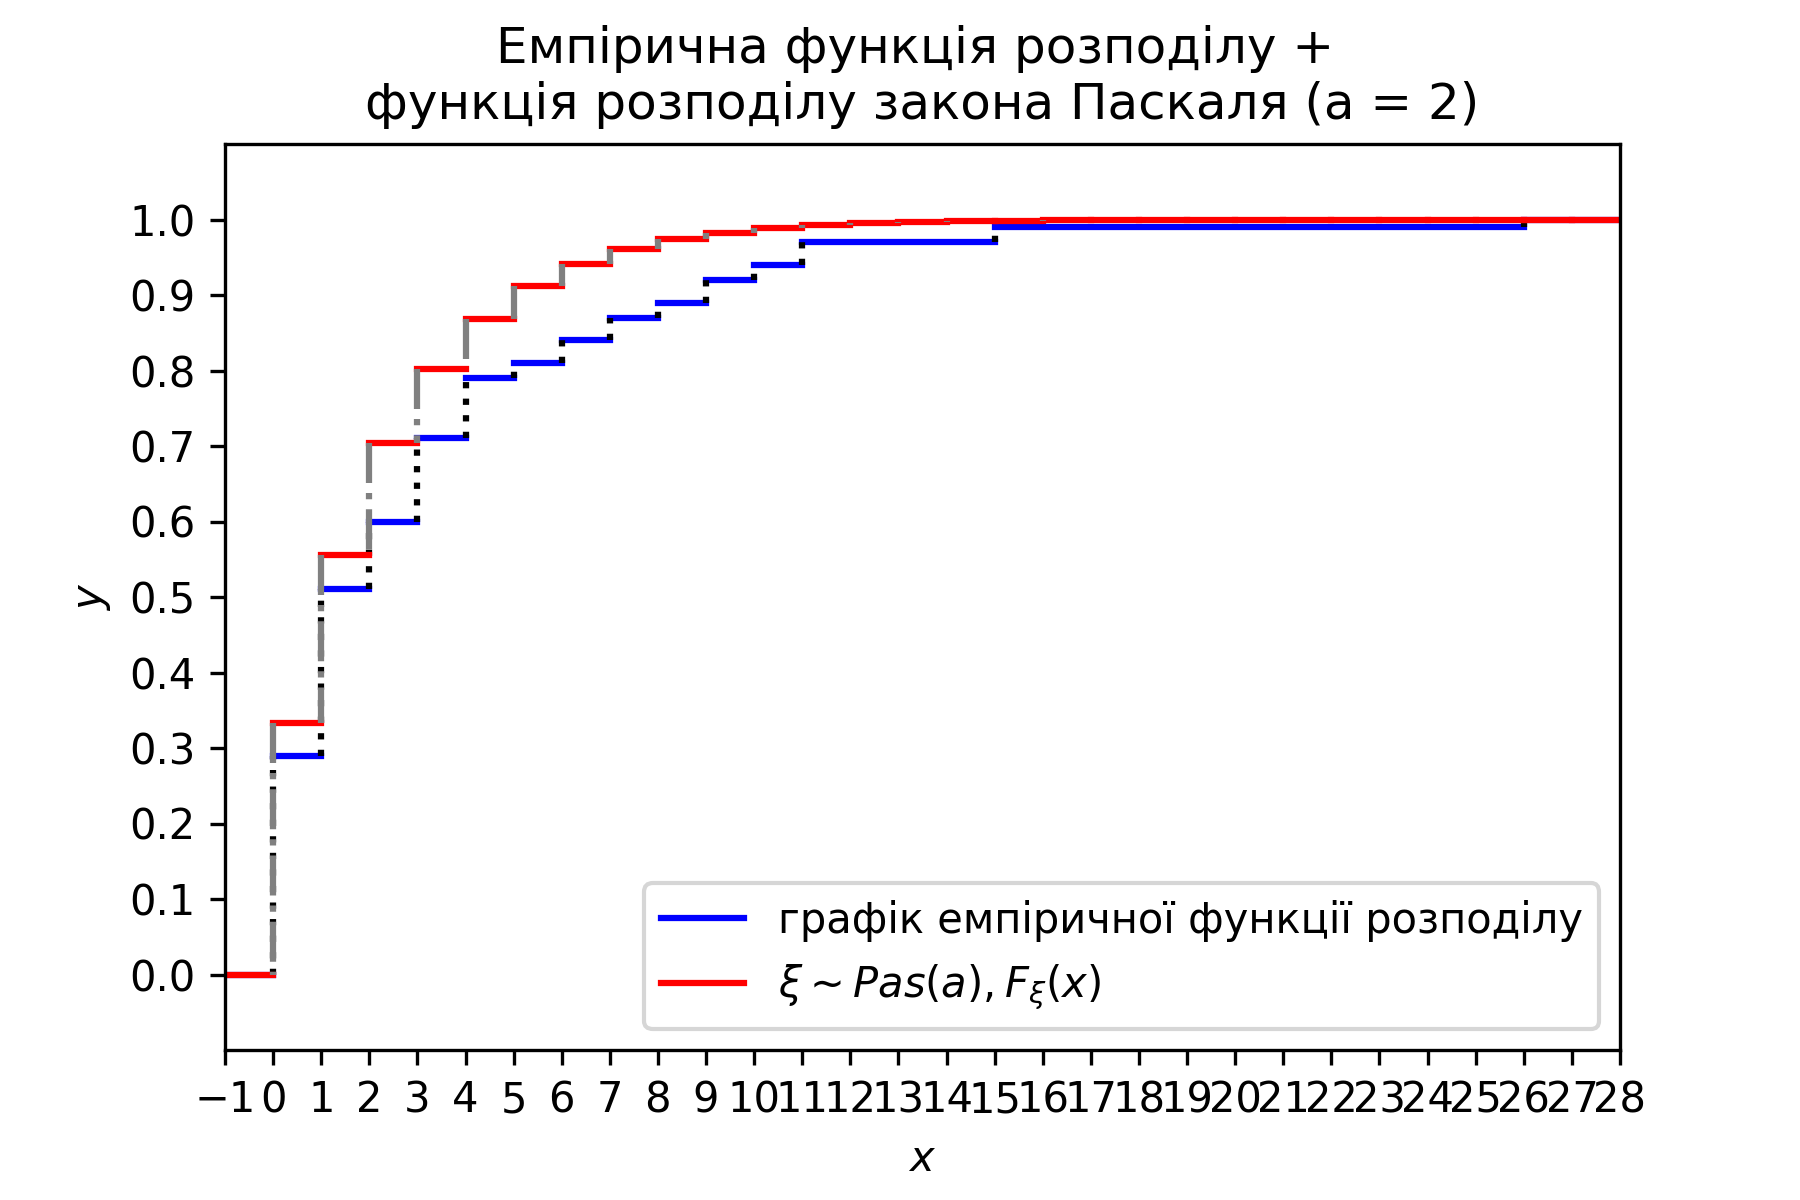
\includegraphics[scale = 0.8]{func+geom3}
\newline
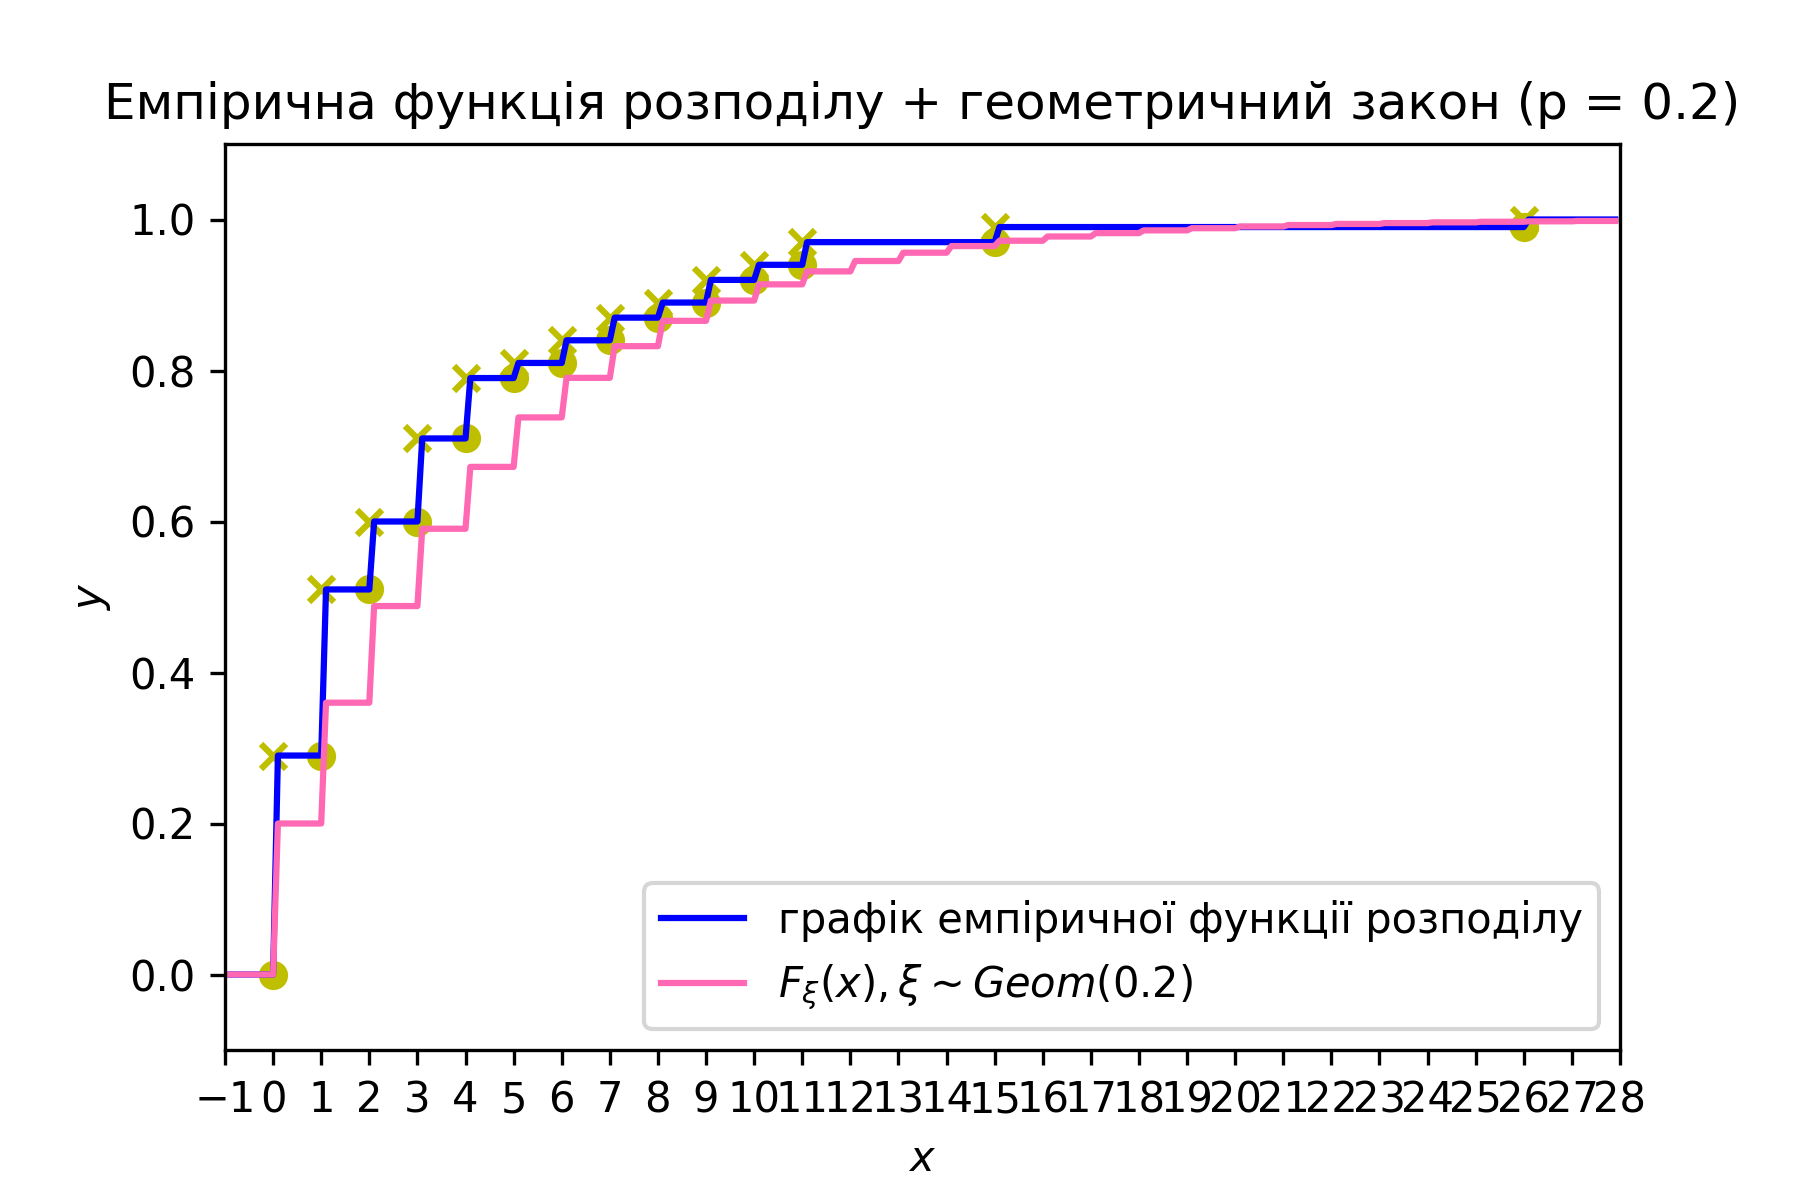
\includegraphics[scale = 0.8]{func+geom2}
\newline
З рисунків вище можна побачити що графік емпіричної функції
розподілу нашої реалізації вибірки певним чином схожий при 
певних значеннях
параметра a на функцію розподілу закону Паскаля.
\section{Обчислення вибіркових характеристик генеральної 
сукупності (медіана, мода, асиметрія)}
Для початку знайдемо $({Mo}_\xi^*)_{\text{знач.}}$ - 
значення вибіркової моди (тієї варіанти, якій відповідає 
найбільша частість). Для знаходження цієї варіанти використаємо
вже побудований дискретний варіаційний ряд (див. стор. 2).
Проаналізувавши варіаційний ряд побачимо, що:
$$({Mo}_\xi^*)_{\text{знач.}} = x_1^* = 0$$
Зауважимо, що випадкова величина $\mu$, розподілена за 
законом Паскаля при будь-яких значеннях параметра a
має моду ${Mo}_\mu = 0$.
\newline
\newline
Знайдемо значення вибіркової медіани $({Me}_\xi^*)_{\text{знач.}}$ 
для нашої реалізації вибірки. Вибірковою медіаною для ДВР називають 
середню за розташуванням варіанту(якщо кількість варіант непарна) 
або середнє арифметичне двох середніх варіант(якщо парна).
З варіаційного ряду (див. ст. 1 
пункт 2), враховуючи те, що кількість варіант - парна, 
знайдемо:$$ ({Me}_\xi^*)_{\text{знач.}} = \frac{x_7^* + x_8^*}
{2} = 6.5 $$
Маємо ще інший спосіб знаходження медіани - знайти першу з варіант, 
для яких накопичена частість перейде за відмітку 0.5. В данному випадку 
такою варіантою буде $x_2^* = 1.$
\newline
Для знаходження значення вибіркової асиметрії спочатку потрібно 
знайти значення вибіркової дисперсії та вибіркового середнього: 
$$\overline{x} = (E^*_{\xi})_{\text{знач.}} = \frac{1}{100} 
\sum_{k = 1}^{14} x_k^* n_k = 3.06$$
За допомогою цього знайдемо значення вибіркової дисперсії:
$$(D^*_{\xi})_{\text{знач.}} = \frac{1}{100} \sum_{k = 1}^{100}
(x_k - 3.06)^2 = 17.1364$$
Отримавши значення вибіркової дисперсії, можна отримати значення
вибіркової асиметрії для даної реалізації вибірки:
$$({As}_{\xi}^*)_{\text{знач.}} = \frac{\frac{1}{100}
\sum_{k = 1}^{100}(x_k - 3.06)^3}{(17.1364)^
{\frac{3}{2}}} = 2.5040$$
\section{Незміщені оцінки математичного сподівання та дисперсії}
$\xi$ - генеральна сукупність, $\vec{\xi} = 
(\xi_1, \xi_2, \dots, \xi_{n})$ - випадкова вибірка, 
n = 100 - об’єм вибірки.  
\newline
За точкову оцінку математичного сподівання візьмемо вибіркове середнє:
$${E_\xi}^* = \frac{1}{n} \sum_{k=1}^{n}\xi_k$$
Перевіримо незміщенність цієї точкової оцінки:
\begin{equation}\label{bias}
  E({E_\xi}^*) = E(\frac{1}{n} \sum_{k=1}^{n}\xi_k) = 
  \frac{1}{n} \sum_{k=1}^{n}E_{\xi_k} = \frac{1}{n}nE_{\xi} 
  = E_\xi
\end{equation}
Відповідно, ця точкова оцінка матсподівання є незміщеною.
\newline
За точкову оцінку дисперсії візьмемо:
$$ {D_{\xi}}^{*} = \frac{1}{n} \sum_{k=1}^n 
(\xi_k - \overline{\xi})^2 = \frac{1}{n}\sum_{k=1}^n
((\xi_k - E_\xi) - (\overline{\xi} - E_\xi))^2 = $$
$$= \frac{1}{n} \sum_{k = 1}^n(\xi_k - E_\xi)^2 - 2(\overline{\xi} 
- E_\xi)\frac{1}{n}\sum_{k=1}^n(\xi_k - E_\xi) + (\overline{\xi} 
- E_\xi)^2 = $$
$$= \frac{1}{n} \sum_{k = 1}^n (\xi_k - E_\xi)^2 - (\overline{\xi} 
- E_\xi)^2$$
Порахуємо матсподівання цієї оцінки:
$$E({D_{\xi}}^{*}) = \frac{1}{n}\sum_{k=1}^n E(\xi_k - E_\xi)^2 
- E(\overline{\xi} - E_\xi)^2 = D_\xi - D_{\overline{\xi}}$$
Бачимо, що ця оцінка - зміщена.
Знайдемо $D_{\overline{\xi}} = \frac{1}{n^2}\sum_{k=1}^n D_{\xi_k} = 
\frac{D_{\xi}}{n}$.
$$E(D_\xi^*) = D_\xi - \frac{D_\xi}{n} = \frac{n-1}{n}D_\xi$$
Тоді оцінка $D^{**}_\xi = \frac{n}{n-1}D_\xi^*$ буде незміщеною 
оцінкою дисперсії.
$$D^{**}_\xi = \frac{n}{n-1} \frac{1}{n} \sum_{k=1}^n 
(\xi_k - \overline{\xi})^2 = \frac{1}{n - 1} \sum_{k=1}^n 
(\xi_k - \overline{\xi})^2$$
Обчислимо значення цих точкових оцінок на данній реалізації вибірки:
$$(E^*_{\xi})_{\text{знач.}} = \frac{1}{100} 
\sum_{k = 1}^{14} x_k^* n_k = 3.06$$
де $x_k^*$ - к-та варіанта, $n_k$ - частота вибірки.
$$(D^{**}_\xi)_\text{знач.} = \frac{1}{99} \sum_{k = 1}^{100}
(x_k - 3.06)^2 = 17.30949494949495$$
\newpage
\section{Гіпотеза про розподіл, за яким отримано вибірку}
Виходячи з того що:
\begin{itemize}
  \item полігон частостей реалізації вибірки схожий на полігон 
  ймовірностей закону Паскаля (див. с. 3-4)
  \item емпірична функцію розподілу реалізації вибірки схожа на
  функцію розподілу закону Паскаля (див. с. 6-7)
  \item мода випадкової величини, розподіленої за законом Паскаля
  дорівнює 0 при будь-яких параметрах закону; в той же самий час 
  значення вибіркової моди для нашої реалізації вибірки також
  дорівнює 0.
  \item в наступному параграфі буде показано, що оцінка математичного 
  сподівання закона Паскаля ${E_\xi}^* = \frac{1}{n} 
  \sum_{k=1}^{n}\xi_k$ є не тільки 
  незміщенною, а й конзистентною та ефективною. Тоді, якщо порівняти 
  полігон частостей даної вибірки та полігон ймовірностей, графік 
  емпіричної функції розподілу та графік функції розподілу закона 
  Паскаля з відповідним параметром(значенням оцінки на данній 
  реалізації вибірки),то вони будуть достатньо схожі(див. 
  наступні рис.)
\end{itemize}
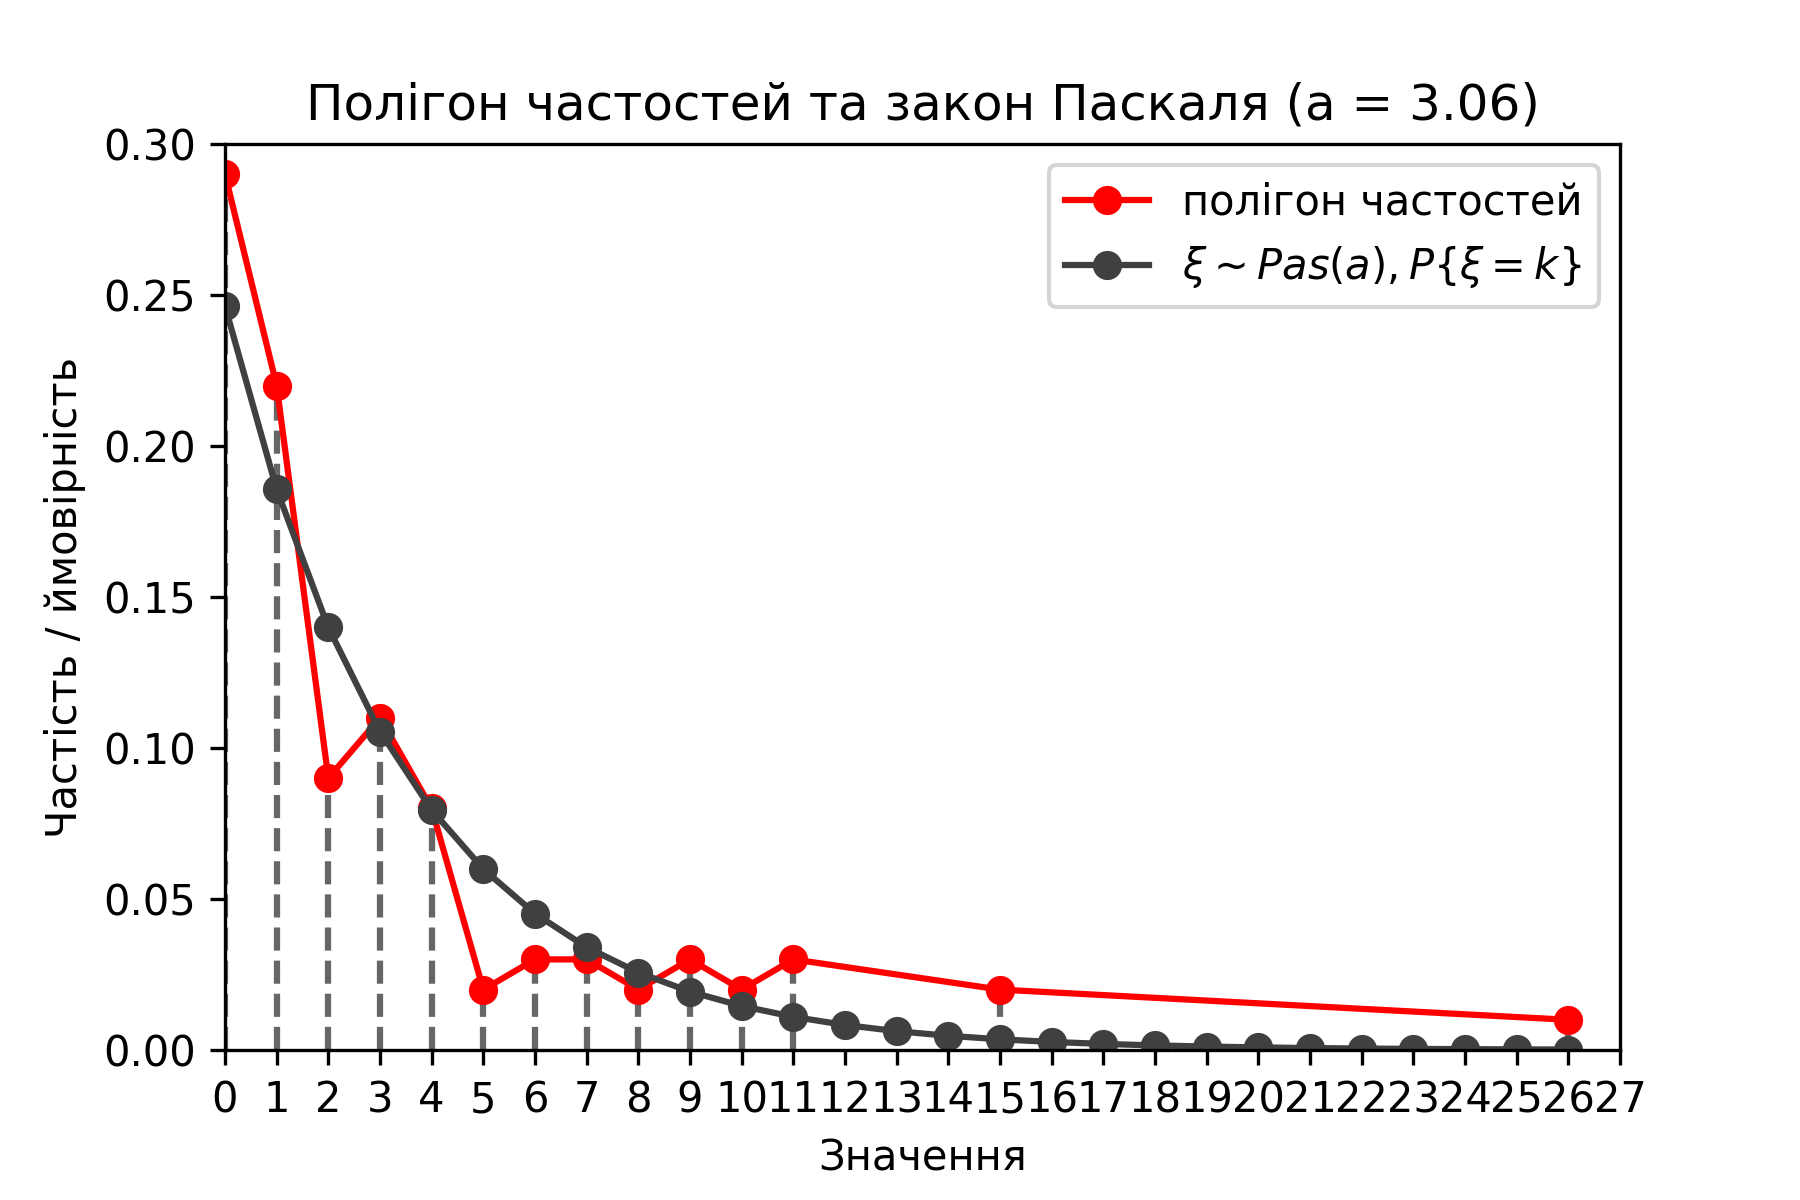
\includegraphics[scale = 0.8]{hypotesis1.png}
\newline
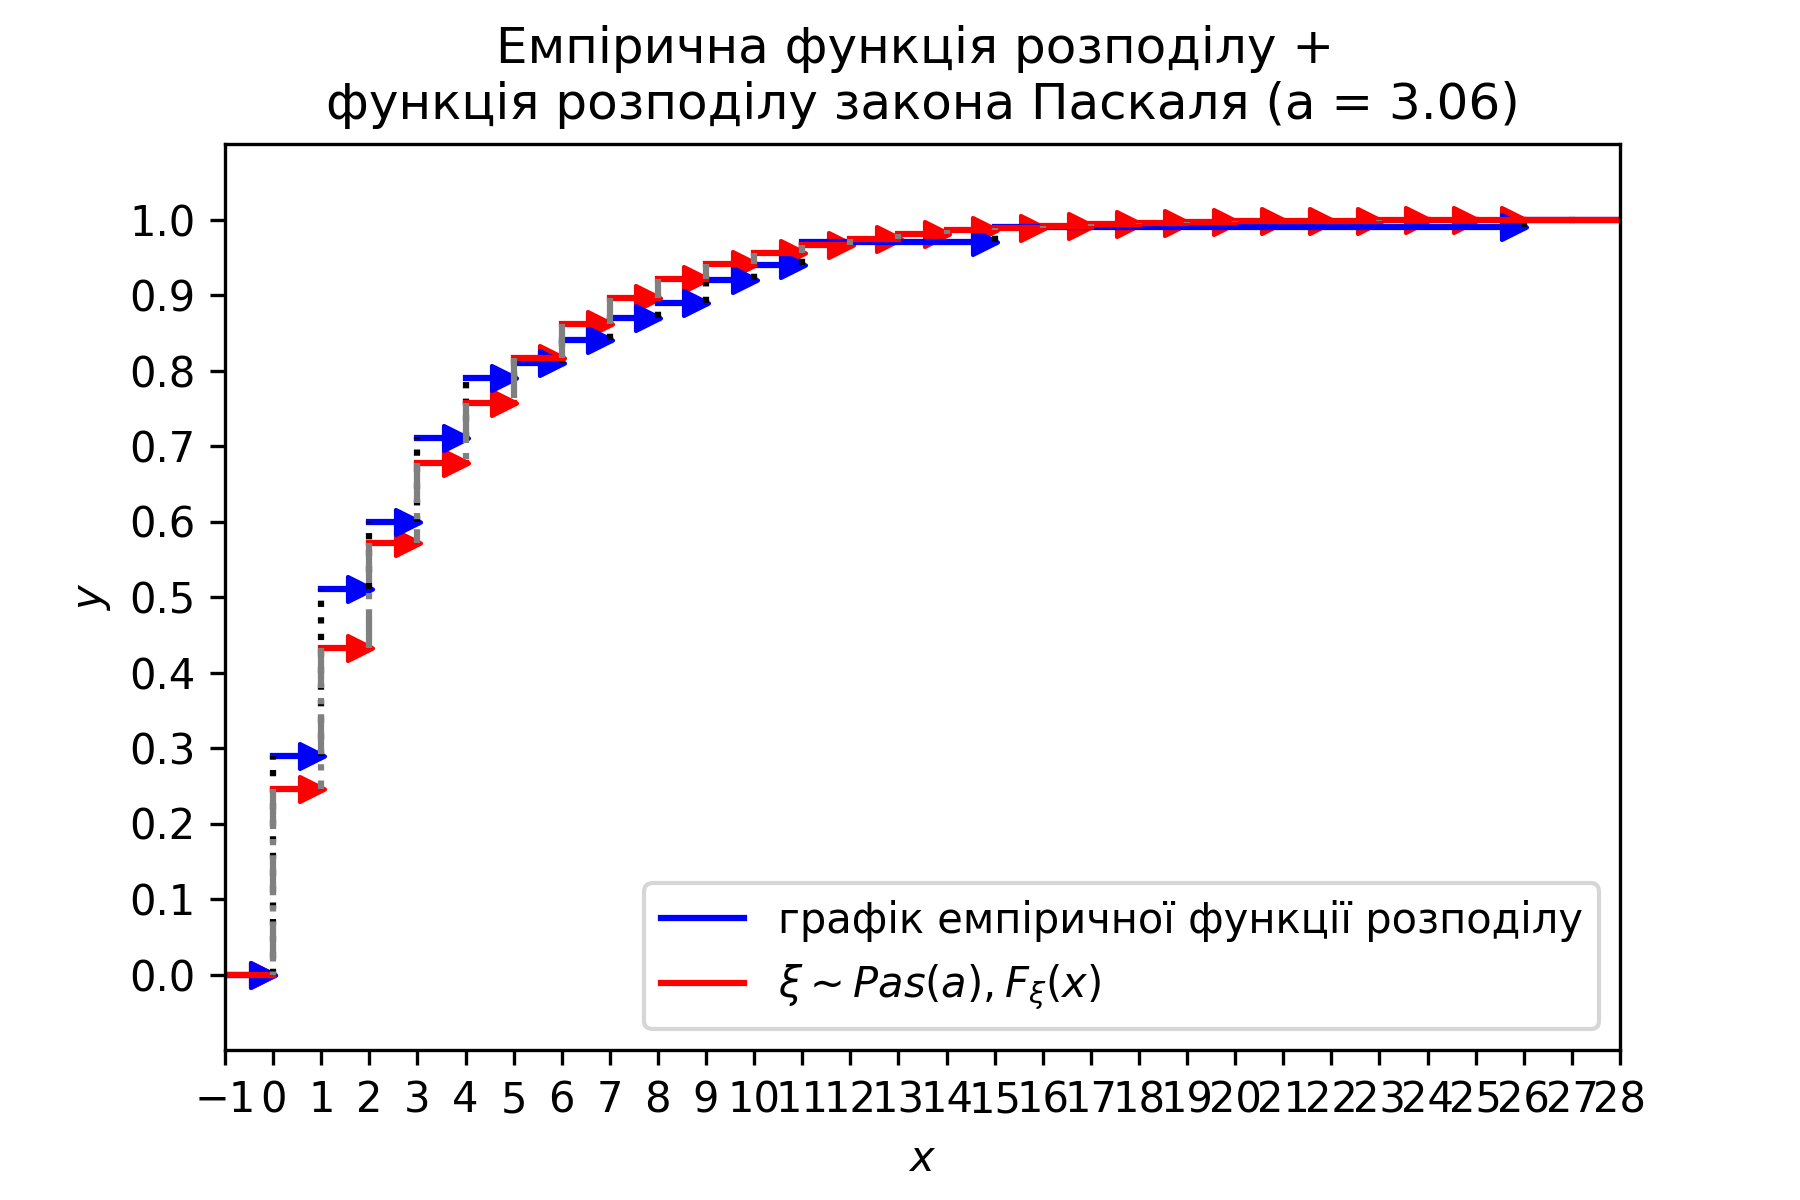
\includegraphics[scale = 0.8]{hypotesis2.png}
\newline
Таким чином висувається гіпотеза, що генеральна сукупність, 
якою породжена данна вибірка, розподілена за законом Паскаля.
\newpage
\section{Точкові оцінки параметру гіпотетичного закону розподілу}
Спочатку скористаємось методом моментів для знаходження точкової 
оцінки параметра a закона Паскаля ( $\mu \sim Pas(a)$ ).
\newline
Прирівняємо емпіричний початковий момент 1-го порядку та математичне 
сподівання випадкової величини, розподіленої за законом Паскаля; 
отримаємо рівняння Пірсона: 
$$E_\mu = E^*_\mu$$
$$E_\mu = a, E^*_\mu = \frac{1}{n} \sum_{k = 1}^n \xi_k$$
\begin{equation}
  (a^*)_\text{мм} = \frac{1}{n} \sum_{k = 1}^n \xi_k
\end{equation}
Отримали статистику - точкову оцінку параметра a закону Паскаля.
\newline
Тепер отримаємо точкову оцінку параметра а за допомогою методу 
максимальної правдоподібності (Фішера). Спочатку знайдемо функцію 
правдоподібності закона Паскаля: 
$$\mathcal{L}( \vec{x}, a ) = \prod_{k = 1}^n \mathbb{P} 
\{\xi = x_k\} = \prod_{k = 1}^n \frac{a^{x_k}}{(1 + a)^{x_k + 1}} = 
\frac{a^{\sum_{k =1}^n x^k}}{(1 + a)^{\sum_{k =1}^n x^k + n}}$$
$$\ln \mathcal{L}( \vec{x}, a ) = (\sum_{k=1}^n x_k)\ln a - 
((\sum_{k=1}^n x_k) + n)\ln(1+a)$$
\begin{equation}
  \frac{\partial\ln \mathcal{L}( \vec{x}, a )}{\partial a} = 
  \frac{1}{a(1+a)}\sum_{k=1}^n x_k - \frac{n}{1+a} = 0
\end{equation}
$$\frac{1}{a(1+a)}\sum_{k=1}^n x_k = \frac{n}{1+a}$$
$$a = \frac{1}{n} \sum_{k=1}^n x_k$$
Отримали оцінку параметра а закона Паскаля методом 
максимальної правдоподібності:
\begin{equation}
  (a^*)_\text{мп} = \frac{1}{n}\sum_{k=1}^n \xi_k
\end{equation}
Перевіримо виконання достатньої умови:
$$\frac{\partial^2\ln \mathcal{L}( \vec{x}, a )}{\partial^2 a} = 
-\frac{1+2a}{a^2(1+a)^2}\sum_{k=1}^n x^k + \frac{n}{(1+a)^2}$$
\begin{equation}
  \left.{\frac{\partial^2\ln \mathcal{L}( \vec{x}, a )}{\partial^2 a}}
  \right|_{a = \frac{1}{n} \sum_{k=1}^n x_k} = -\frac{n^2}{(1+\frac{1}{n} \sum_{k=1}^n x_k)^2}\left({\frac{1}{\frac{1}{n} \sum_{k=1}^n x_k} + 1}\right) < 0
\end{equation}
Достатня умова виконана.
\newline
Обома методами отримали однакову оцінку параметра а:
$$(a^*)_{\text{мм}} = (a^*)_{\text{мп}} = a^* = \frac{1}{n}
\sum_{k=1}^n \xi_k = \overline{\xi}$$
Перевіримо властивості цієї оцінки:
\begin{enumerate}
  \item \textbf{Незміщенність.} Вже доведена раніше (див. 2 cтор.9)
  \item \textbf{Конзистентність.} Так як $\{\xi_k\}$ - i.i.d\footnote{
    i.i.d. - Independent and identically distributed random variables 
    -  незалежні та однаково розподілені випадкові величини
  }
  , для $\forall \xi_k :E_{\xi_k} = a < \infty, D_{\xi_k} = a^2 + a - 
  \text{рівномірно обмежені}$, то за ЗВЧ
  \newline 
  $a^*\xrightarrow[n\to\infty]{\mathbb{P} }E_{a^*} = a$.
  А це і означає що оцінка конзистентна.
  \newpage
  \item \textbf{Ефективність.} Розглянемо вираз 
  $\frac{\partial\ln \mathcal{L}( \vec{\xi}, a )}{\partial a}$.
  Його вже було знайдено раніше ( див. 4 стор. 13 ).
  $$\frac{\partial\ln \mathcal{L}( \vec{\xi}, a )}{\partial a} = 
  \frac{1}{a(1+a)}\sum_{k=1}^n \xi_k - \frac{n}{1+a} = $$
  $$= \frac{n}{a(1+a)}(\frac{1}{n}\sum_{k=1}^n \xi_k - a) = $$
  $$= C(n, a)(a^* - a)$$
  Таким чином, за наслідком з нерівності Рао-Крамера, оцінка $a^* = 
  \frac{1}{n}\sum_{k=1}^n \xi_k$ є ефективною.
  \item \textbf{Асимптотична нормальність.} Знайдемо дисперсію 
  цієї оцінки:
  $$D(a^*) = D(\frac{1}{n}\sum_{k=1}^n \xi_k) = \bigg|\xi_k - 
  \text{незалежні}\bigg| 
  = $$
  $$= \frac{1}{n^2} \sum_{k=1}^nD_{\xi_k} = \frac{a^2 + a}{n}$$
  Перевіримо за визначенням асимптотичну нормальність оцінки:
  $$\frac{a^* - E_{a^*}}{\sqrt{D_{a^*}}} = 
  \frac{(\frac{1}{n}\sum_{k=1}^n \xi_k) - a}{\sqrt{\frac{a^2 + a}{n}}} = 
  \frac{\sum_{k=1}^n \frac{\xi_k - a}{n}}{\sqrt{\frac{a^2 + a}{n}}} = $$
  $$= \frac{\sum_{k=1}^n(\xi_k - a)}{\sqrt{n(a^2 + a)}} = 
  \frac{\sum_{k=1}^n(\xi_k - a)}{\sqrt{\sum_{k=1}^n(a^2 + a)}} =$$
  $$= \frac{\sum_{k=1}^n(\xi_k - E_{\xi_k})}{\sqrt{
  \sum_{k=1}^nD_{\xi_k}}} \xrightarrow[n\to\infty]{\mathbb{F} } 
  N(0, 1)$$
  Останній граничний перехід має місце згідно з наслідку з теореми 
  Ляпунова для однаково розподілених випадкових величин.
  Таким чином, оцінка $a^*$ є асимптотично нормальною.
\end{enumerate}
Таким чином, маємо незміщенну, конзистентну, ефективну та 
асимптотично нормальну оцінку параметра a закона Паскаля.
\section{Перевірка гіпотези про розподіл}
Перевірка гіпотези про розподіл генеральної сукупності буде здійснюватись 
за допомогою критерію $\chi^2$ (Пірсона)  з рівнем значущості $\alpha = 0.05$.
\newline
Критерій $\chi^2$ (Пірсона) заснований на використанні теореми Пірсона:
\begin{theorem}[Пірсона]
  Якщо складна гіпотеза $H_0$ про закон розподілу ГС справджується, то 
  статистика критерію $\eta = \sum_{i=1}^r\frac{(n_i - np_i)^2}{np_i}$ 
  прямує в слабкому сенсі до розподілу $\chi^2$ (Пірсона) з r-s-1 
  ступенями вільності, де s - кількість параметрів гіпотетичного закону, 
  що були оцінені, $n_i$ - кількість значень реалізації вибірки, що потрапили в 
  $X_i, i = \overline{1, r}$

\end{theorem}
Висунемо гіпотезу $H_0: \xi \sim Pas(3.06)$. Згідно нашої гіпотези, 
генеральна сукупність може приймати такі значення: $\{0, 1, 2, \dots\}$.
Розіб'ємо цю множину на такі підмножини $X_i$, $i = \overline{0,5}$:

\begin{multicols}{2}
  \begin{itemize}
    \item $X_0 = \{0\}$
    \item $X_1 = \{1\}$
    \item $X_2 = \{2\}$
    \item $X_3 = \{3\}$
    \item $X_4 = \{4, 5\}$
    \item $X_5 = \{6, 7, \dots\}$
  \end{itemize}
\end{multicols}
\newpage
Обчислимо ймовірності $p_i = \mathbb{P}(\xi \in X_i/H_0)$ та 
$n_i$ - кількість значень реалізації вибірки, що потрапили в 
$X_i$.
\newline
\begin{tabular}{|l|l|l|l|l|l|l|}
  \hline
  $X_i$ & $\{0\}$ & $\{1\}$ & $\{2\}$ & $\{3\}$ & $\{4, 5\}$ & 
  $\{6, 7, \dots\}$ \\
  \hline
  $p_i$ & $0.2463$ & $0.1856$ & $0.1399$ & $0.1055$ & 
  $0.1394$ & $0.1833$\\
  \hline
  $n\cdot p_i$ & $24.63$ & $18.56$ & $13.99$ & $10.55$ & 
  $13.94$ & $18.33$\\
  \hline
  $n_i$ & 29 & 22 & 9 & 11 & 10 & 19 \\
  \hline
\end{tabular}
\newline
\newline
Бачимо, що $\sum_{i = 0}^{5}p_i = 1$, r = 6, і виконується умова 
\newline
$\forall i$ : 
$np_i \geq 10$.
Обчислимо значення статистики:
$$\eta = \sum_{i=1}^r\frac{(n_i - np_i)^2}{np_i}$$
$$\eta_\text{знач.} = \frac{(29 - 24.63)^2}{24.63} + 
\frac{(22 - 18.56)^2}{18.56} + \frac{(9 - 13.99)^2}{13.99} + $$
$$+ \frac{(11 - 10.55)^2}{10.55} + \frac{(10 - 13.94)^2}{13.94} + 
\frac{(19 - 18.33)^2}{18.33} \approx 4.35007$$
$r - s - 1 = 6 - 1 - 1 = 4, \alpha = 0.05$, тому за таблицею розподілу 
Пірсона знайдемо значення $t_{0.05, 4} = 9.5$. Бачимо, що 
$\eta_\text{знач.} < t_{0.05, 4}$. Робимо висновок, що на рівні 
значущості 0.05 дані не суперечать висунутій гіпотезі про те, що 
генеральна сукупність розподілена за законом Паскаля($\xi 
\sim Pas(3.06)$).
\newpage
\section{Довірчий інтервал для параметра гіпотетичного закону 
розподілу}
За рівень надійності довірчого інтервалу беремо $\gamma = 0.95$.
За точкову оцінку параметра a візьмемо $a^* = \frac{1}{n}
\sum_{k=1}^n \xi_k$. Для цієї оцінки вже була знайдена її дисперсія 
та доведена асимптотична нормальність оцінки. 
\newline
Побудуємо такий довірчий інтервал, що:
$$\mathbb{P} \{|a^* - a| < \varepsilon \} = \gamma = 0.95$$ 
З асимптотичної нормальності оцінки випливає те, що:
$$\mathbb{P}\{\frac{|a^* - a|}{\sqrt{D_{a^*}}} < t \} \approx 
\Phi(t) + \frac{1}{2},$$
де $\Phi(t) = \frac{1}{\sqrt{2\pi}}\int_{0}^{t} e^{-\frac{x^2}{2}} \,\mathrm{d}x $.
За допомогою таблиці значень функції Лапласа приблизно 
знайдемо таке t, що $\Phi(t) + \frac{1}{2} = 0.95$; $\Phi(t) = 0.45$;
$t \approx 1.65$.
\newline
Тепер розв'яжемо нерівність $\frac{|a^* - a|}{\sqrt{D_{a^*}}} < t$ 
відносно а, враховуючи те, що $D_{a^*} = \frac{a^2 + a}{n}$:
$$|a^* - a| < t\sqrt{\frac{a^2 + a}{n}}$$
$$(a^* - a)^2 < t^2(\frac{a^2 + a}{n})$$
$$(a^*)^2 - 2aa^* + a^2 < t^2(\frac{a^2 + a}{n})$$
$$a^2(1 - \frac{t^2}{n}) + a(-2a^* - \frac{t^2}{n}) + (a^*)^2 < 0$$
$$\mathcal{D} = (2a^* + \frac{t^2}{n})^2 - 4(a^*)^2(1 - \frac{t^2}{n})$$
$$a_{1,2} = \frac{(2a^* + \frac{t^2}{n}) \pm 
\sqrt{(2a^* + \frac{t^2}{n})^2 - 4(a^*)^2(1 - \frac{t^2}{n})}}
{2(1 - \frac{t^2}{n})}$$
$$a \in \left(\frac{(2a^*_{\text{зн}} + \frac{t^2}{n}) - 
\sqrt{(2a^*_{\text{зн}} + \frac{t^2}{n})^2 - 4(a^*_{\text{зн}})^2(1 - \frac{t^2}{n})}}
{2(1 - \frac{t^2}{n})}, \right.$$
$$\left.\frac{(2a^*_{\text{зн}} + \frac{t^2}{n}) + 
\sqrt{(2a^*_{\text{зн}} + \frac{t^2}{n})^2 - 4(a^*_{\text{зн}})^2(1 - \frac{t^2}{n})}}
{2(1 - \frac{t^2}{n})}\right)$$
Підставивши значення, отримаємо:
$$a \in \left(2.5616, 3.7576\right) \text{з ймовірністю }0.95$$
\newpage
\section{Висновки}
Під час виконання даної розрахункової роботи було проведено обробку 
деякої реалізації вибірки, побудовано дискретний варіаційний ряд 
та емпіричну функцію розподілу, зображено їх геометрично у вигляді 
полігону частостей та графіку емпіричної функції розподілу, 
порівняно їх з полігоном ймовірностей та графіком функції розподілу 
відповідно закону Паскаля при деяких значеннях його параметра, 
обчислено значення вибіркової медіани, моди та асиметрії данної 
реалізації вибірки, знайдено незміщені точкові оцінки матсподівання 
та дисперсії. Наслідком цих дій було висунення гіпотези про розподіл 
за законом Паскаля генеральної сукупності, з якої була отримана 
реалізація вибірки. Було знайдено таку точкову оцінку параметра 
гіпотетичного закону розподілу, що є не тільки незміщенною, а й 
конзистентною, ефективною та асимптотично нормальною. За допомогою критерію 
$\chi^2$(Пірсона) було виявлено, що на рівні значущості 0.05 дані не 
суперечать висунутій гіпотезі про те, що генеральна сукупність 
розподілена за законом Паскаля з параметром a = 3.06. Останнім було 
отримано довірчий інтервал (2.5616, 3.7576) для параметра а 
з рівнем надійності 0.95.
\end{document}
